\newpage
\section{Проектування програмного продукту}
\subsection{Концептуальне проектування}
\bigbreak
Діаграму концептуальних класів наведено на рис. 2.1.

\noindent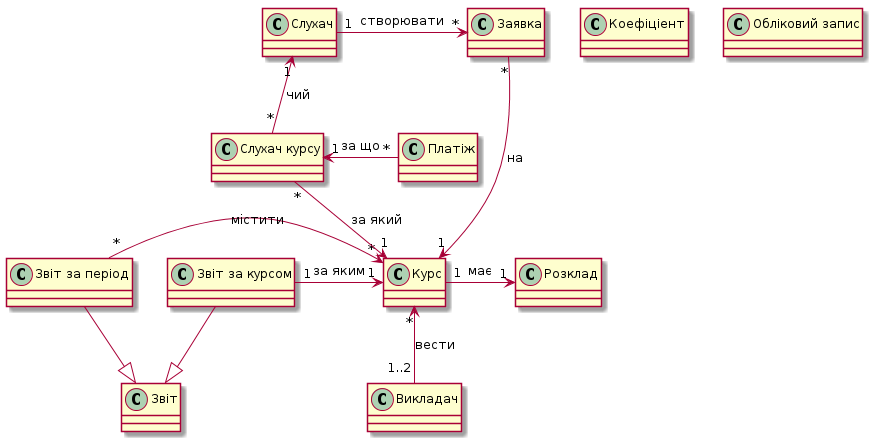
\includegraphics[width=17cm]{pp_pw3_conc.png}
\imglabel{Діаграма концептуальних класів}

Клас <<Курс>> характеризується високою зв'язністю [8], тобто це головний клас у системі.
\bigbreak
\subsection{Логічне проектування}
\bigbreak
Діаграму програмних класів наведено на рис. А.5.

Як і на діаграмі концептуальних класів, клас Course характеризується високою зв'язністю та має найбільшу кількість атрибутів. Також високу зв'язність має AccessControl, що відповідає висновку з пункту 1.2.1.

\bigbreak
\subsection{База даних}
\def\dbhead{
 \hline
 \Centering Ключ &
 \Centering Назва &
 \Centering Ім'я поля &
 \Centering Тип &
 \Centering NULL &
 \Centering Дод.\\
 \hline
}
\tablefirsthead{\dbhead}
\tablehead{\multicolumn{4}{l}{Продовження таблиці \thesection .\thetabcount} \\\hline\dbhead}
\def\dbtable#1#2#3{
 \tablabel{Опис структури таблиці <<#1>> (#2)}\\
 \begin{supertabular}{|p{1.2cm}|p{3.5cm}|p{3cm}|p{2.8cm}|p{1.2cm}|p{4.3cm}|}
 #3
 \hline
 \end{supertabular}
 \\[-3mm]
}
\newcommand{\tabheader}[2]{
 #1 \emph{(#2)}
}
\setlength{\tabcolsep}{3pt}
\dbtable{Слухачі}{listeners}{
PK & Ідентифікатор & idListener & int(6) & Ні & A\_I\\
 & Ім'я & Name & varchar(30) & Так & \\
 & Прізвіще & Surname & varchar(30) & Ні & \\
 & По батькові & Patronymic & varchar(30) & Так & \\
 & Університетська група & UGroup & varchar(6) & Так & \\
 & Телефон & Phone & varchar(20) & Так & \\
 & E-mail & Email & varchar(40) & Так & \\
FK & Ким змінено & affectedBy & varchar(32) & Ні & \\
}
\dbtable{Курси}{courses}{
PK & Ідентифікатор & idCourse & int(6) & Ні & A\_I\\
 & Назва & Name & varchar(50) & Ні & \\
 & Опис & Description & varchar(400) & Так & \\
 & Ознака індивідуального курсу & isIndividual & bit(1) & Ні & \\
FK & Викладач & idTeacher & int(6) & Так & \\
FK & Другий викладач & idTeacher2 & int(6) & Так & \\
 & Ціна & Price & decimal(10,2) & Так & \\
 & Стан & state & tinyint(1) & Ні & 0..2 (Йде набір, набрано, завершений)\\
FK & Ким змінено & affectedBy & varchar(32) & Ні & \\
}
\dbtable{Слухачі курсу}{Course\_Listeners}{
PK & Ідентифікатор & idCL & int(6) & Ні & A\_I\\
FK & Курс & idCourse & int(6) & Ні & \\
FK & Слухач & idListener & int(6) & Ні & \\
 & Оцінка & mark & tinyint(3) & Так & \\
FK & Ким змінено & affectedBy & varchar(32) & Ні & \\
}
\dbtable{Платежі}{payments}{
PK & Ідентифікатор & idPayment & int(6) & Ні & A\_I\\
FK & Слухач курсу & idCL & int(6) & Ні & \\
 & Кошти & delta & int(6) & Ні & \\
 & Мітка часу & timestamp & timestamp & Ні & CURRENT\_\newline TIMESTAMP\\
}
\dbtable{Викладачі}{teachers}{
PK & Ідентифікатор & idTeacher & int(6) & Ні & A\_I\\
 & Ім'я & Name & varchar(30) & Так & \\
 & Прізвіще & Surname & varchar(30) & Ні & \\
 & По батькові & Patronymic & varchar(30) & Так & \\
 & Телефон & Phone & varchar(20) & Так & \\
 & E-mail & Email & varchar(40) & Так & \\
FK & Ким змінено & affectedBy & varchar(32) & Ні & \\
FK & Вчений ступінь & degree & tinyint(2) & Так & \\
}
\dbtable{Розцінки}{prices}{
PK & Ідентифікатор & degree & tinyint(2) & Ні & A\_I\\
 & Вчений ступінь & deglab & varchar(30) & Ні & \\
 & Зарплата & salary & decimal(10,2) & Ні & \\
}
\dbtable{Коефіціенти}{coefficients}{
PK & Назва & name & varchar(64) & Ні & \\
 & Мітка & label & varchar(128) & Так & \\
 & Значення & value & float & Так & \\
}
\dbtable{Заняття}{lessons}{
PK & Ідентифікатор & idLesson & int(11) & Ні & A\_I\\
FK & Курс & idCourse & int(11) & Ні & \\
 & Дата & date & date & Так & \\
 & Час початку & time & time & Ні & \\
 & Тип & type & tinyint(1) & Ні & 0..1 (Лекція, Практика)\\
}
\dbtable{Користувачі}{users}{
PK & Логін & login & varchar(32) & Ні & \\
 & Хеш паролю & password & text & Ні & \\
 & Сіль & salt & text & Ні & \\
 & Тип & type & tinyint(1) & Ні & 0..2 (Оператор, Адміністратор, Переглядач)\\
 & Ключ сесії & sessionid & text & Так & \\
}
\bigbreak
\subsection{Оцінка алгоритмічної складності}
\bigbreak
На рис. А.6 зазначено складну операцію розрахунку вартості за даними з БД. Вона реалізується наступним SQL-запитом:

{ \fontsize{11pt}{12pt} \selectfont
\begin{verbatim}
SELECT ifnull(s1,0)*ifnull(c1,0)+ifnull(s2,0)*ifnull(c2,0) FROM ((
 SELECT salary as s1 FROM prices WHERE degree IN (
  SELECT degree FROM teachers WHERE idTeacher IN (
   SELECT idTeacher FROM courses WHERE idCourse=?
))) s1 LEFT OUTER JOIN (
 SELECT salary as s2 FROM prices WHERE degree IN(
  SELECT degree FROM teachers WHERE idTeacher IN (
   SELECT idTeacher2 FROM courses WHERE idCourse=?
))) s2 ON 1=1) LEFT OUTER JOIN ((
 SELECT count(*) as c1 FROM lessons WHERE idCourse=? AND type=0
) c1 ON 1=1 LEFT OUTER JOIN (
 SELECT count(*) as c2 FROM lessons WHERE idCourse=? AND type=1
) c2) ON 1=1;
\end{verbatim}
}

\FloatBarrier
План виконання запиту:
\begin{enumerate}
\item Вибірка вмісту таблиці courses
\item Проекція кортежів за значенням атрибуту idCourse
\item Проекція атрибутів за атрибутом idCourse
\item Вибірка вмісту таблиці teachers
\item Проекція кортежів за значенням атрибуту idTeacher
\item Проекція атрибутів за атрибутом degree
\item Вибірка вмісту таблиці prices
\item Проекція кортежів за значенням атрибуту degree
\item Проекція атрибутів за атрибутом salary
\item Використання вибірки з п. 1.
\item Проекція кортежів за значенням атрибуту idCourse
\item Проекція атрибутів за атрибутом idCourse
\item Використання вибірки з п. 4.
\item Проекція кортежів за значенням атрибуту idTeacher
\item Проекція атрибутів за атрибутом degree
\item Використання вибірки з п. 7.
\item Проекція кортежів за значенням атрибуту degree
\item Проекція атрибутів за атрибутом salary
\item Вибірка вмісту таблиці lessons
\item Проекція кортежів за значенням атрибуту idCourse
\item Проекція кортежів за значенням атрибуту type
\item Підрахунок кортежів
\item Використання проекції з п. 20.
\item Проекція кортежів за значенням атрибуту type
\item Підрахунок кортежів
\item З'єднання результатів пп. 9 та 18.
\item З'єднання результатів пп. 22 та 25.
\item З'єднання результатів пп. 26 та 27.
\item Розрахунок математичного виразу за результатом п. 28.
\end{enumerate}

Операції проекції кортежів у пп. 2, 3, 5, 6, 8, 9, 11, 12, 14, 15, 17 та 18 повинні повертати один кортеж. Пошук у таблицях courses та teachers відбувається за первинним ключем, а таблиця prices складається з кількох кортежів. Для проекцій з пп. 20, 21 та 24 доцільно створити у таблиці lessons індекс за атрибутом idCourse. За атрибутом type індекс недоцільний, оскільки проекції за ним відбуваються не з усієї таблиці, а можливих значення тільки два. SQL-запит для створення індексу:

{ \fontsize{11pt}{12pt} \selectfont
\begin{verbatim}
CREATE INDEX course_of_lesson ON lessons (idCourse);
\end{verbatim}
}

Циклів в алгоритмах на рис. А.6 та А.7 немає, тож їх складність --- \emph{O(1)} [9].

\bigbreak
\subsection{Опис зовнішних інтерфейсів}
\bigbreak
Інтерфейс користувача побудовано із використанням бібліотеки Kendo UI, дизайн визначається наявними для неї темами оформлення. Доступні самостійні концептуальні класи присутні у головному меню та розташовані за частотою використання: найактивніша робота проводиться зі слухачами та курсами, викладачі та користувачі заповнюються на початку роботи і потім змінюються рідко, звіти здаються рідко, розцінки та коефіціенти змінюються у виключних випадках. В кінці головного меню розміщено кнопку виходу з системи. Екран авторизації є окремим та лаконічним, містить лише форму та кнопку перемикання форм реєстрації та входу.

Для роботи серверної частини системи потрібен веб-сервер Apache 2.x, інтерпретатор PHP5 не нижче 5.4, СКБД MySQL або MariaDB 5. Для користування клієнтською частиною потрібен web-браузер із підтримкою EcmaScript 5; тестування проводиться у поточних версіях браузерів Mozilla Firefox та Chromium для десктопу.

Система може працювати у межах однієї машини, через локальну мережу та через мережу Інтернет, в залежності від мережевих підключень та налаштувань машини, на якій встановлено серверну частину. Підключення, відповідно, може здійснюватись будь-яким доступним дротовим або бездротовим каналом підключення до локальної мережі або мережі Інтернет: Ethernet, Wi-Fi, ADSL, HSPA, Dial-up та ін. Оскільки звіти генеруються у форматі PDF, для їх перегляду потрібна програма --- переглядач PDF: Mozilla Firefox, Google Chrome, Adobe Reader, Foxit Reader тощо. [10] Для друку потрібен принтер, підключений безпосередньо до машини, на якій відкрито файл звіту, або доступний для неї через мережу.
